\notechapter{N-20260602}{Matrix Decompositions: LU, Cholesky, Full Rank, and SVD}

\section{Why decompositions are algorithms}
A decomposition rewrites a matrix into factors that are easier to compute with.  LU reduces a system to triangular solves; Cholesky uses positive definiteness; full-rank decomposition exposes rank; SVD exposes singular directions.

\section{Doolittle LU}
If \(A\in\mathbb C^{n\times n}\) can be written as
\[
  A=LU,
\]
where \(L\) is unit lower triangular and \(U\) is upper triangular, this is the Doolittle or LU decomposition.

\section{Existence and uniqueness}
If the first \(n-1\) leading principal minors of \(A\) are nonzero, then \(A=LU\) exists.  If \(A\) is nonsingular, the decomposition is unique.  The condition says that Gaussian elimination without row exchange never meets a zero pivot.

\section{Elimination matrices}
At step \(k\), an elimination matrix \(L_k\) zeros entries below the pivot.  After all steps,
\[
  L_{n-1}\cdots L_1A=U,\qquad
  A=L_1^{-1}\cdots L_{n-1}^{-1}U.
\]
The product of the inverses is the lower triangular factor.

\section{Doolittle formulas}
Comparing \(A=LU\) gives
\[
  u_{kj}=a_{kj}-\sum_{t=1}^{k-1}l_{kt}u_{tj},\qquad j\ge k,
\]
\[
  l_{ik}=\frac{1}{u_{kk}}\left(a_{ik}-\sum_{t=1}^{k-1}l_{it}u_{tk}\right),\qquad i>k.
\]
The pivot \(u_{kk}\) must be nonzero.

\section{Pivoting}
If a pivot is zero or small, row exchange is needed.  With partial pivoting,
\[
  PA=LU,
\]
where \(P\) is a permutation matrix.  Pivoting controls large multipliers and improves numerical stability.

\section{Storage of LU}
The upper triangle stores \(U\); the strictly lower triangle stores the multipliers \(l_{ij}\).  The diagonal of \(L\) is omitted because it is all ones.

\section{Cholesky decomposition}
If \(A\) is Hermitian positive definite, there is a unique lower triangular \(L\) with positive diagonal such that
\[
  A=LL^H.
\]
Solving \(Ax=b\) becomes
\[
  Ly=b,\qquad L^Hx=y.
\]
Cholesky costs about \(\frac13n^3+O(n^2)\), roughly half of LU.

\section{Cholesky example}
For
\[
  A=\begin{bmatrix}4&2\\2&5\end{bmatrix},
\]
we obtain
\[
  L=\begin{bmatrix}2&0\\1&2\end{bmatrix},\qquad A=LL^T.
\]

\section{Full-rank decomposition}
If \(\operatorname{rank}A=r>0\), a full-rank decomposition is
\[
  A=FG,\qquad F\in\mathbb C^{m\times r},\quad G\in\mathbb C^{r\times n},
\]
with both factors rank \(r\).  It always exists and is not unique.

\section{Hermite standard form}
Row operations reduce \(A\) to a Hermite-style form \(H\).  If pivot columns are \(j_1,\ldots,j_r\), choose \(F\) as the corresponding columns of \(A\), and \(G\) as the nonzero rows of \(H\).  Then \(A=FG\).

\section{Singular values}
The singular values of \(A\) are
\[
  \sigma_i=\sqrt{\lambda_i(A^HA)}.
\]
Unitary equivalence preserves singular values.

\section{Singular value decomposition}
If \(\operatorname{rank}A=r\), then
\[
  A=U\begin{bmatrix}\Sigma&0\\0&0\end{bmatrix}V^H,\qquad
  \Sigma=\operatorname{diag}(\sigma_1,\ldots,\sigma_r).
\]
SVD says that \(A\) rotates, stretches along orthogonal axes, and rotates again.

\section{SVD geometry}
\begin{figure}[H]
\centering
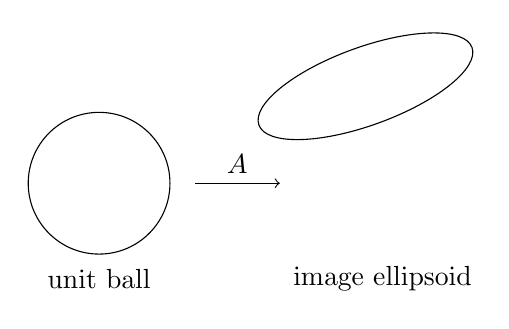
\begin{tikzpicture}[scale=0.9]
  \draw (0,0) circle (1);
  \node at (0,-1.35) {unit ball};
  \draw[->] (1.35,0) -- (2.55,0) node[midway,above] {$A$};
  \draw[rotate=20] (4,0) ellipse (1.6 and 0.55);
  \node at (4,-1.35) {image ellipsoid};
\end{tikzpicture}
\caption{SVD describes the image of the unit ball as an ellipsoid.}
\end{figure}

\section{Which decomposition matches the matrix}

\begin{center}
\small
\begin{tabularx}{\textwidth}{@{}lYY@{}}
\toprule
Decomposition & Hypothesis or signal & What it gives\\
\midrule
\(LU\) & square system without severe pivot trouble & triangular solves\\
\(PA=LU\) & row exchanges needed & stable Gaussian elimination\\
\(A=LL^H\) & Hermitian positive definite & fast symmetric solve\\
\(A=FG\) & \(\operatorname{rank}A=r\) & factorization through an \(r\)-dimensional space\\
\(A=U\Sigma V^H\) & arbitrary rectangular matrix & singular directions and rank profile\\
\bottomrule
\end{tabularx}
\end{center}
The choice should be driven by structure rather than by habit.  Cholesky is inappropriate without positive definiteness; ordinary LU may need pivoting when a small or zero pivot appears; a full-rank decomposition records the actual dimension through which the linear map factors.  The SVD is the most geometric option: it says that the unit ball is rotated, stretched by the singular values, and rotated again.  This is why the nonzero singular values detect rank and why small singular values signal directions in which solving or inversion will be unstable.
